%%%%%%%%%%%%%%%%%%%%%%%%%%%%%%%%%%%%%%%%%
% The Legrand Orange Book
% LaTeX Template
% Version 3.1 (February 18, 2022)
%
% This template originates from:
% https://www.LaTeXTemplates.com
%
% Authors:
% Vel (vel@latextemplates.com)
% Mathias Legrand (legrand.mathias@gmail.com)
%
% License:
% CC BY-NC-SA 4.0 (https://creativecommons.org/licenses/by-nc-sa/4.0/)
%
% Compiling this template:
% Compiling this template:
% This template uses biber for its bibliography and makeindex for its index.
% When you first open the template, compile it from the command line with the 
% commands below to make sure your LaTeX distribution is configured correctly:
%
% 1) pdflatex main
% 2) makeindex main.idx -s indexstyle.ist
% 3) biber main
% 4) pdflatex main x 2
%
% After this, when you wish to update the bibliography/index use the appropriate
% command above and make sure to compile with pdflatex several times 
% afterwards to propagate your changes to the document.
%
%%%%%%%%%%%%%%%%%%%%%%%%%%%%%%%%%%%%%%%%%

%----------------------------------------------------------------------------------------
%	PACKAGES AND OTHER DOCUMENT CONFIGURATIONS
%----------------------------------------------------------------------------------------

\documentclass[
        11pt, % Default font size, select one of 10pt, 11pt or 12pt
	%fleqn, % Left align equations(控制公式是否行偏左)
	a4paper, % Paper size, use either 'a4paper' for A4 size or 'letterpaper' for US letter size
	%oneside, % Uncomment for oneside mode, this doesn't start new chapters and parts on odd pages (adding an empty page if required), this mode is more suitable if the book is to be read on a screen instead of printed
]{LegrandOrangeBook}

% Book information for PDF metadata, remove/comment this block if not required 
\hypersetup{
	pdftitle={Title}, % Title field
	pdfauthor={Author}, % Author field
	pdfsubject={Subject}, % Subject field
	pdfkeywords={Keyword1, Keyword2, ...}, % Keywords
	pdfcreator={LaTeX}, % Content creator field
}

\addbibresource{sample.bib} % Bibliography file

\definecolor{ocre}{RGB}{243, 102, 25} % Define the color used for highlighting throughout the book
% \definecolor{ocre}{RGB}{0, 0, 0} % Define the color used for highlighting throughout the book

\chapterimage{orange1.jpg} % Chapter heading image
\chapterspaceabove{6.5cm} % Default whitespace from the top of the page to the chapter title on chapter pages
\chapterspacebelow{6.75cm} % Default amount of vertical whitespace from the top margin to the start of the text on chapter pages

%----------------------------------------------------------------------------------------
%	以下是我们自己添加的额外packages
%----------------------------------------------------------------------------------------

%----------------------------------------------------------------------------------------
%	让pdf纸张变成护眼色,保护眼睛。启用\pagecolor命令时生效。
\usepackage{xcolor} % For defining and using colors
\definecolor{mygreen}{RGB}{205, 222, 194} % Define a custom green color for eye protection
% \pagecolor{mygreen} % Set page background color to custom green
%----------------------------------------------------------------------------------------

\usepackage[colorinlistoftodos]{todonotes}

%贺立添加的包--------------------------------------------------------------
\usepackage{graphicx}
\usepackage{quantikz}
\usepackage{csquotes}
%\usepackage{mathbbol}
%\usepackage{mdframed}
\usepackage{xcolor}
\usepackage{ulem}
\usepackage[thicklines]{cancel}
\usepackage{tocbibind} % 加载宏包以添加目录到目录中
\usepackage{caption}
\captionsetup[figure]{labelsep=space}

% 定义自定义的方框样式
% \mdfdefinestyle{mystyle}{
% 	roundcorner=10pt,
% 	backgroundcolor=blue!10,
% 	frametitlerule=true,
% 	frametitlebackgroundcolor=blue!20,
% }
%----------------------------------------------------------------------

%\newtheorem{theorem}{Theorem}
%\newtheorem{remark}{Remark}
%\newtheorem{property}{Property}
%\newtheorem{definition}{Definition}
%\newtheorem{example}{Example}
%\newtheorem{corollary}{Corollary}
%\newtheorem{lemma}{Lemma}
%\newtheorem{postulate}{Postulate}
%\newtheorem{proposition}{Proposition}
%\renewcommand{\thefootnote}{\fnsymbol{footnote}} %注脚符号的注脚方式

%----------------------------------------------------------------------------------------
%   向\input{}命令追加文件搜索路径
\makeatletter % 允许在命令名中使用@字符
\providecommand*{\input@path}{} % 定义一个新的命令\input@path,如果该命令不存在,则初始化为空
\g@addto@macro\input@path{ % 向\input@path命令追加文件搜索路径
{Part I Mathematical Foundations/Linear algebra/} 
{Part I Mathematical Foundations/Other Math/}
{Part II Quantum Mechanics/}
{Part III Quantum Computation/Quantum circuits/}
{Part III Quantum Computation/The quantum Fourier transform and its applications/}
{Part III Quantum Computation/Quantum search algorithms/}
{Part IV Notes of Papers/By Laizhijian/}
{Part V Other Notes/Simon's Algorithm/}
{Part V Other Notes/Inexact Infeasible Interior Point Method/}
{Part V Other Notes/A Concise Introduction to Quantum Computing/}
}
\makeatother % 恢复对@字符的正常处理,不再允许在命令名中使用
%----------------------------------------------------------------------------------------

\begin{document}

%----------------------------------------------------------------------------------------
%	TITLE PAGE
%----------------------------------------------------------------------------------------

\titlepage % Output the title page
	{
\includegraphics[width=\paperwidth]{background.pdf}} % Code to output the background image, which should be the same dimensions as the paper to fill the page entirely; leave empty for no background image
	{ % Title(s) and author(s)
		\centering\sffamily % Font styling
		{\Huge\bfseries
            Lai's ideas for \\
            Quantum Computation and Optimization
            \par} % Book title
		\vspace{16pt} % Vertical whitespace
		{\LARGE A Study Note\par} % Subtitle
		\vspace{24pt} % Vertical whitespace
		{\huge\bfseries
            Zhijian Lai
            \par} % Author name
	}

% %----------------------------------------------------------------------------------------
% %	COPYRIGHT PAGE
% %----------------------------------------------------------------------------------------

% \thispagestyle{empty} % Suppress headers and footers on this page

% ~\vfill % Push the text down to the bottom of the page

% \noindent Copyright \copyright\ 2022 Goro Akechi\\ % Copyright notice

% \noindent \textsc{Published by Publisher}\\ % Publisher

% \noindent \textsc{\href{https://www.latextemplates.com/template/legrand-orange-book}{book-website.com}}\\ % URL

% \noindent Licensed under the Creative Commons Attribution-NonCommercial 4.0 License (the ``License''). You may not use this file except in compliance with the License. You may obtain a copy of the License at \url{https://creativecommons.org/licenses/by-nc-sa/4.0}. Unless required by applicable law or agreed to in writing, software distributed under the License is distributed on an \textsc{``as is'' basis, without warranties or conditions of any kind}, either express or implied. See the License for the specific language governing permissions and limitations under the License.\\ % License information, replace this with your own license (if any)

% \noindent \textit{First printing, March 2022} % Printing/edition date

%----------------------------------------------------------------------------------------
%	TABLE OF CONTENTS
%----------------------------------------------------------------------------------------

\pagestyle{empty} % Disable headers and footers for the following pages

\tableofcontents % Output the table of contents

% \listoffigures % Output the list of figures, comment or remove this command if not required

% \listoftables % Output the list of tables, comment or remove this command if not required

\pagestyle{fancy} % Enable default headers and footers again

\cleardoublepage % Start the following content on a new page

%----------------------------------------------------------------------------------------
%	SECTIONING EXAMPLES CHAPTER
%----------------------------------------------------------------------------------------

\chapterimage{orange2.jpg} % Chapter heading image
\chapterspaceabove{6.75cm} % Whitespace from the top of the page to the chapter title on chapter pages
\chapterspacebelow{7.25cm} % Amount of vertical whitespace from the top margin to the start of the text on chapter pages

%------------------------------------------------

% ==========================  正文开始  ==========================

\chapter{Lai's Ideas}

\section{Policy Gradient Algorithm for Binary Optimization \cite{chen2023monte}}\label{sec:prob_model}

We study the binary optimization problem:
\begin{equation}
    \text{min } f(x) \text{ s.t. } x \in \{0,1\}^n. \tag{1}
\end{equation}
Let $\mathcal{X}^* \subset \{0,1\}^n$ be the set of optimal solutions.

\begin{enumerate}
    \item Suppose that we know the ideal distribution
\begin{equation}
    q^{}(x)= 
\begin{cases}\frac{1}{\left|\mathcal{X}^{}\right|}, & x \in \mathcal{X}^{}, \\ 0, & x \notin \mathcal{X}^{},
\end{cases}  \quad \forall x \in \{0,1\}^{n}.
\end{equation}
If we sample according to $q^{}$, then we will definitely get an optimal solution of (1). However, the optimal points set $\mathcal{X}^{}$ is unknown.
    \item To approximate $q^*$, we introduce the Gibbs distributions, 
\begin{equation}
    q_\lambda(x) = \frac{1}{Z_\lambda} \exp \left(-\frac{f(x)}{\lambda}\right),  \quad \forall x \in \{0,1\}^{n},
\end{equation}
with parameter $\lambda > 0$. Here, $Z_{\lambda}$ is the normalization factor. We can show that,\footnote{For proofs, see \cite[eq. (4)]{chen2023monte}} for all points $x \in\mathcal \{0,1\}^n$, 
\begin{equation}
    q_\lambda(x) \rightarrow q^*(x), \quad \text { as } \lambda \rightarrow 0.
\end{equation}
However, denominator $Z_{\lambda}$ is practically uncomputable. Also, $q_{\lambda}$ is hard to sample when $f$ owns a rough landscape.
    \item For now, a small $\lambda$ was set in advance. The policy distribution $p_\theta(x)$ with parameters $\theta$ is designed to approximate $q_\lambda$ to enable efficient sampling\footnote{How to sample? MCPG paper used the whole Section 3 to realize this goal.}. We measure their difference using 
\begin{equation}
    \mathrm{KL}\left(p_\theta \| q_\lambda\right)=\sum_{x \in \mathcal{B}_n} p_\theta(x) \log \frac{p_\theta(x)}{q_\lambda(x)}
\end{equation}
and try to find the best $\theta^*$ by solving $\min_\theta \mathrm{KL}(p_\theta \| q_\lambda)$, leading to:\footnote{For proofs, see \cite[eq. (5)]{chen2023monte}}
\begin{equation}
    \min \quad L(\theta)=\mathbb{E}_{p_\theta}[f(x)]+\lambda \mathbb{E}_{p_\theta}[\log p_\theta(x)]=\mathbb{E}_{p_\theta}[f(x)+\lambda \log p_\theta(x)].
\end{equation}
The policy gradient of $L(\theta)$ is
\begin{equation}
    \nabla_{\theta} L(\theta)=\mathbb{E}_{p_{\theta}}[(f(x)+\lambda \log p_{\theta}(x) + b ) \nabla_{\theta} \log p_{\theta}(x)], \quad \forall \text{ constant } b \in \mathbb{R}
\end{equation}
and its Monte Carlo estimate is
\begin{equation}
    \bar{g}(\theta, S) = \frac{1}{|S|}\sum_{x \in S} (f(x)+\lambda \log p_\theta(x)) \nabla_\theta \log p_\theta(x),
\end{equation}
where $S \subset \{0,1\}^n$ is a sample set from $p_\theta(x)$.
    \item Finally, we propose a prototype of policy gradient algorithm: \\
Choose an initial $\theta^{0}$. For $t=0,1,2,\dots,$
    \begin{enumerate}
    \item $p_{\theta^{t}}$ indicates where potential good solutions might be.
    \item Take a sample set $S^{t}$ from $p_{\theta^{t}}$.
    \item Update the parameter $\theta$ as $\theta^{t+1}=\theta^t-\eta^t \bar{g}\left(\theta^t, S^t\right)$, where $\eta^t$ is the step size.
    \item $t \leftarrow t+1.$
    \end{enumerate}
\end{enumerate}

\textbf{How to choose policy distribution?}
In \cite{chen2023monte}, they choose the parameterized policy distribution follows the multivariate Bernoulli distribution:
\begin{equation}
    p_\theta(x)=\prod_{i=1}^n \mu_i^{\left(1+x_i\right) / 2}\left(1-\mu_i\right)^{\left(1-x_i\right) / 2}, \mu_i=\frac{1}{1+e^{-\theta_i}}.
\end{equation}
One can choose a neutral network, like policy network used in reinforcement learning.

\textbf{Compare to VQA.}
I feel VQA is a special case of above, where we let $p_{\theta}$ to be the measurement of output state of a quantum circuit. However, we often only minimize the term $g(\theta)=\mathbb{E}_{p_\theta}[f(x)]$  in $L(\theta)$, without considering the entropy regularization of $p_\theta$.

\section{Our Idea: Applying TRPO and PPO}

\subsection{Trust Region Policy Optimization (TRPO)}

\begin{align}
    L(\theta)
    =\mathbb{E}_{p_\theta}\left[f(x)\right]
    =\mathbb{E}_{p_{\theta^{\prime}}}\left[ \frac{p_\theta(x)}{p_{\theta^{\prime}}(x)} f(x)\right].
\end{align}

Let $\pi_\theta$ denote a policy with parameters $\theta$. The theoretical TRPO update is:
\begin{equation}
\begin{aligned}
& \theta_{k+1}=\arg \max _\theta \mathcal{L}\left(\theta_k, \theta\right) \\
& \text { s.t. } \mathrm{KL}\left(p_\theta \| p_{\theta_k} \right) \leq \Delta
\end{aligned}
\end{equation}
where $\mathcal{L}\left(\theta_k, \theta\right)$ is the surrogate advantage, a measure of how policy $\pi_\theta$ performs relative to the old policy $\pi_{\theta_k}$ using data from the old policy:
\begin{equation}
    \mathcal{L}\left(\theta_k, \theta\right)
=\mathbb{E}_{p_{\theta_k}}\left[ \frac{p_\theta(x)}{p_{\theta_k}(x)} f(x)\right]
\end{equation}

\subsection{Proximal Policy Optimization (PPO)}

\begin{enumerate}
    \item \textbf{PPO-penalty}
    \begin{equation}
    \theta_{k+1}=\arg \max _\theta
    \mathcal{L}\left(\theta_k, \theta\right)
    =\mathbb{E}_{p_{\theta_k}}\left[ \frac{p_\theta(x)}{p_{\theta_k}(x)} f(x)\right] + \beta \cdot \mathrm{KL}\left(p_\theta \| p_{\theta_k} \right)
\end{equation}
    \item \textbf{PPO-clip}
    \begin{equation}
    \theta_{k+1}=\arg \max _\theta
    \mathcal{L}\left(\theta_k, \theta\right)
    =\mathbb{E}_{p_{\theta_k}}\left[ \min \left(\frac{p_\theta(x)}{p_{\theta_k}(x)} f(x), \operatorname{clip}\left(\frac{p_\theta(x)}{p_{\theta_k}(x)}, 1-\epsilon, 1+\epsilon\right) f(x)\right) \right]
\end{equation}
\end{enumerate}

\section{VQA and QAOA (adapted from Lin \cite{grange2023introduction})}

\subsection{VQA}

The main idea of a VQA is as follows.

\begin{enumerate}
    \item For any parameter $\theta \in \mathbb{R}^d,$ $U(\theta) \in \mathcal{M}_{2^n}(\mathbb{C})$ is a $n$-qubits quantum circuit that can be executed on the quantum computer.
    \item Fixing the input state $\left|0_n\right\rangle$, we obtain the output state  $|\psi (\theta) \rangle = U(\theta)\left|0_n\right\rangle$. When $|\psi (\theta) \rangle$ is measured, it results in a discrete distribution probability $p_\theta(x)$, namely,
\begin{equation}
    p_\theta(x)=\left|\left\langle x|U(\theta)| 0_n\right\rangle\right|^2, \quad \forall x \in \{0,1\}^{n}.
\end{equation}
    \item A guiding function $g(\theta)=G\left(p_{\theta}, f\right)$ for a given function $G$ that is constructed from $f$ and $p_{\theta}$. For example, such $g$ can be    
\begin{equation}
    g(\theta)=\sum_{x \in\{0,1\}^n} p_\theta(x) f(x).
\end{equation}
    Eventually, this cost value is given to the classical optimizer $\mathcal{A}$, which outputs a new parameter in order to minimize $g$.
\end{enumerate}

\begin{figure}
    \centering
    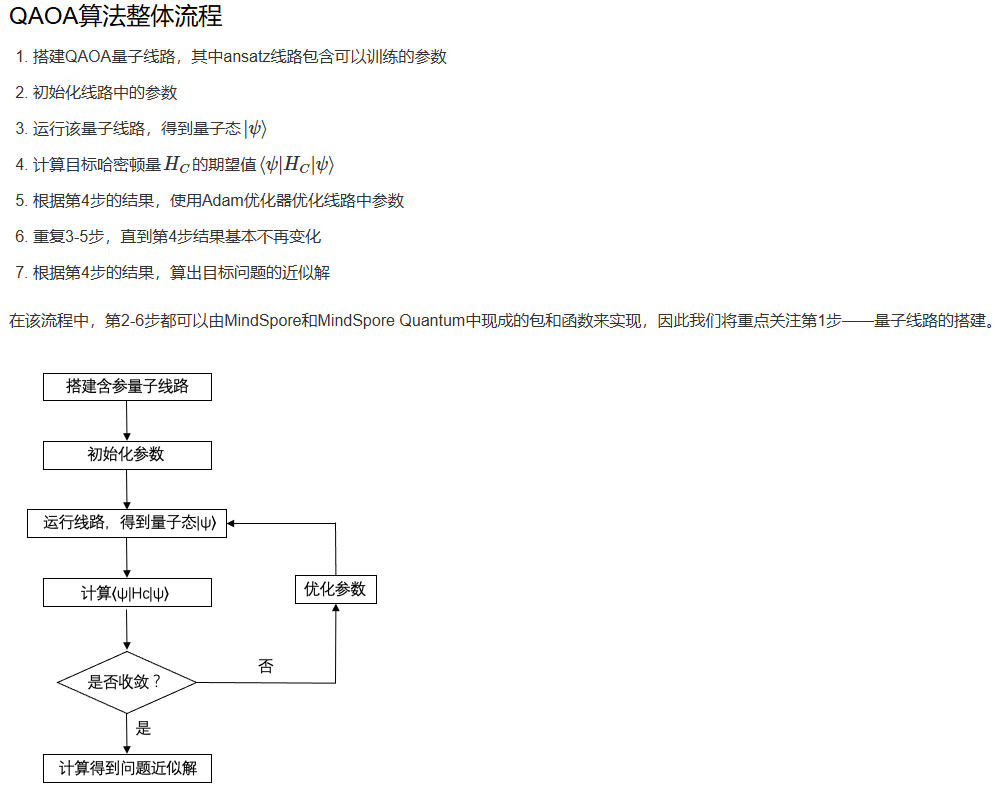
\includegraphics[width=1\linewidth]{Images/mindspore-qaoa.png}
    \caption{\href{https://www.mindspore.cn/mindquantum/docs/zh-CN/r0.9/case_library/quantum_approximate_optimization_algorithm.html}{MindSpore Quantum, QAOA } }
\end{figure}

\subsection{QAOA --- a Special Circuit for Polynomial $f$}

\paragraph{Problem Reformulation}
We assume that the function $f$ is \textit{polynomial}. Since $x$ is a binary variable, we can write
\begin{equation}
    f(x)
=\sum_{i_1=0}^1 \sum_{i_2=0}^1 \cdots \sum_{i_n=0}^1 a_{i_1 i_2 \cdots i_n} x_1^{i_1} x_2^{i_2} \cdots x_n^{i_n}
=\sum_{i=\left(i_1, \ldots ,i_n\right) \in\{0,1\}^n} a_i \prod_{k=1}^n x_k^{i_k}.
\end{equation}
We transform this $\{0,1\}$ problem into a $\{-1,1\}$ problem, which leads to:
\begin{equation}
    \min _{z \in\{-1,1\}^{n}} f_{ \pm}(z)=\sum_{\alpha=\left(\alpha_{1}, \ldots \alpha_{n}\right) \in\{0,1\}^{n}} h_{\alpha} \prod_{i=1}^{n} z_{i}^{\alpha_{i}}.
\end{equation}
\paragraph{Hamiltonian of Objective Function}
We define the $2^n$ by $2^n$ matrix $H_{f}$ (called "Hamiltonian") as
\begin{equation}
    H_{f}:=\sum_{\alpha=\left(\alpha_{1}, \ldots \alpha_{n}\right) \in\{0,1\}^{n}} h_{\alpha} \bigotimes_{i=1}^{n} Z_{i}^{\alpha_{i}},
\end{equation}
where $Z=\left(\begin{array}{cc}1 & 0 \\ 0 & -1\end{array}\right), Z^{0}=I$ and $Z^{1}=Z$. We note $Z_{i}$ the application of $Z$ to qubit $i$. By \cite[Proposition 32]{grange2023introduction}, we can show that 
\begin{equation}
    H_{f}|x\rangle=f(x)|x\rangle, \quad \forall x \in \{0,1\}^{n}.
\end{equation}
Therefore, we have that $\langle x | H_{f}|x\rangle=f(x)$. Under some output state $|\psi(\theta)\rangle$, we write
\begin{equation}
    \langle H_{f} \rangle := \langle \psi(\theta)| H_{f}|\psi(\theta)\rangle =\sum_{x \in\{0,1\}^n} p_\theta(x) f(x)= g(\theta).
\end{equation}
To see the above equality, note that $\forall x \in\{0,1\}^n, p_\theta(x)=|\left\langle x| \psi(\theta)\rangle\right|^2=|\psi(\theta)_x|^2$, where $| \psi(\theta)\rangle= \sum_{x \in\{0,1\}^n} \psi(\theta)_x | x\rangle$.

% 注意,这里要重点参考NCBOOK的投影测量的概念。这里的可观测量就是Hf。注意Hf的特征值就是对角线上的f(x)的值。所以测量得到的就是f(x)。并且,Hf的特征向量就是标注正交基底,其中投影算子Pm= | m > < m |,m就是二进制label。经计算,p(m)=<psi \ Pm \ psi> = p_theta(x). 注意,这里m,x,i都是同样的标准基底的index。

\paragraph{Example}
We illustrate this transformation on a small example with $n=2$. Let us consider the problem
\begin{equation}
    \min _{x \in\{0,1\}^{2}} f(x)=x_{1}+2 x_{2}-3 x_{1} x_{2}.
\end{equation}
Using (20), the equivalent $\{-1,1\}$-problem is
\begin{equation}
    \min _{z \in\{-1,1\}^{2}} f_{ \pm}(z)=\frac{1}{4} z_{1}-\frac{1}{4} z_{2}-\frac{3}{4} z_{1} z_{2}+\frac{3}{4}.
\end{equation}
Thus, the Hermitian matrix associated with the problem is
\begin{equation}
    H_{f}=\frac{1}{4} Z \otimes I-\frac{1}{4} I \otimes Z-\frac{3}{4} Z \otimes Z+\frac{3}{4} I \otimes I
\end{equation}
To illustrate (21), we compute the eigenvalue of the canonical basis state $|10\rangle$.
\begin{equation}
\begin{aligned}
H_{f}|10\rangle & =\frac{1}{4}(Z \otimes I)|10\rangle-\frac{1}{4}(I \otimes Z)|10\rangle-\frac{3}{4}(Z \otimes Z)|10\rangle+\frac{3}{4}(I \otimes I)|10\rangle \\
& =-\frac{1}{4}|10\rangle-\frac{1}{4}|10\rangle+\frac{3}{4}|10\rangle+\frac{3}{4}|10\rangle \\
& =|10\rangle \\
& =f(1,0)|10\rangle
\end{aligned}
\end{equation}
because $f(1,0)=1$.

\paragraph{Quantum Circuit of QAOA}
Define the two types of quantum gates:
\begin{enumerate}
    \item $e^{-i  \gamma H_{f}}$, for any $\gamma \in \mathbb{R}$.
    \item $e^{-i \beta  H_{B} }$, for any $\beta \in \mathbb{R}$. Here, $H_{B}=\sum_{i=1}^{n} R_{X, i}(\pi).$
\end{enumerate}
The quantum circuit of QAOA is given by
\begin{equation}
    U(\boldsymbol{\gamma}, \boldsymbol{\beta})
= e^{-i \beta_p H_B} e^{-i \gamma_p H_{f}} \ldots e^{-i \beta_1 H_B} e^{-i \gamma_1 H_{f}} H^{\otimes n},
\end{equation}
where $(\boldsymbol{\gamma}, \boldsymbol{\beta})=\left(\gamma_{1}, \ldots, \gamma_{p}, \beta_{1}, \ldots, \beta_{p}\right) \in \mathbb{R}^{2 p}$ and $p$ is called depth.

\section{Quantum Measurement Postulate (adapted from Lin \cite{lin2022lecture}) }

Without loss of generality, we only discuss a special type of quantum measurements called the \textbf{projective measurement}. 

\begin{theorem}[Quantum measurement postulate]
In a finite dimensional setting (namely, an $n$-qubits system), a quantum \textbf{observable} always corresponds to an (arbitrary) Hermitian matrix $M$, which has the spectral decomposition
\begin{equation}
    M=\sum_m \lambda_m P_m .
\end{equation}
Here $\lambda_m \in \mathbb{R}$ are the eigenvalues of $M$, and $P_m$ is the projection operator (i.e., $P_m^2=P_m$) onto the eigenspace associated with $\lambda_m$.

When a quantum state $|\psi\rangle$ is measured by a quantum observable $M$, the outcome of the measurement is always an eigenvalue $\lambda_m$, with probability
\begin{equation}
    p_m=\left\langle\psi\left|P_m\right| \psi\right\rangle.
\end{equation}
After the measurement, the quantum state becomes
\begin{equation}
    |\psi\rangle \rightarrow \frac{P_m|\psi\rangle}{\sqrt{p_m}}.
\end{equation}
Note that this is not a unitary process!
\end{theorem}

\begin{remark}
    We just need to accept this assumption/postulate and don't need to ask yourself why, unless you want to learn the whole of quantum mechanics.
\end{remark}

In order to evaluate the expectation value of a quantum observable $M$, we first use the resolution of identity: $\sum_m P_m=I$. This implies the normalization condition,
\begin{equation}
    \sum_m p_m=\sum_m\left\langle\psi\left|P_m\right| \psi\right\rangle=\langle\psi \mid \psi\rangle=1.
\end{equation}
Together with $p_m \geq 0$, we find that $\left\{p_m\right\}$ is indeed a probability distribution. Note that
\begin{equation}
    \mathbb{E}_\psi(M)=\sum_m \lambda_m p_m=\sum_m \lambda_m\left\langle\psi\left|P_m\right| \psi\right\rangle=\left\langle\psi\left|\left(\sum_m \lambda_m P_m\right)\right| \psi\right\rangle=\langle\psi|M| \psi\rangle.
\end{equation}

\begin{definition}[Expectation value of the measurement]
    The expectation value of the measurement outcome under a quantum observable $M$ w.r.t. to sate $|\psi\rangle$ is
\begin{equation}
    \langle M \rangle:=\langle M \rangle_{\psi}:= \mathbb{E}_\psi(M)=\langle\psi|M| \psi\rangle.
\end{equation}
\end{definition}

\begin{remark}
    A widely used phrase, to 'measure in a basis $|i\rangle$ ', where $|i\rangle$ form an orthonormal basis, simply means to perform the projective measurement with projectors $P_i=|i\rangle\langle i|$.
\end{remark}

\subsection{Summary of Lai's Understanding}

The current understanding is as follows: % 目前的理解如下:
\begin{enumerate}
    \item Given a quantum state to be observed. Any Hermitian operator M can be used as an observable to measure this quantum state. The specific methods and experimental approaches are to be determined by physicists and engineers.
    \item Each measurement yields an eigenvalue of $M$ as outcome. The eigenvalues of Hermitian operators are always real numbers, which aligns with the concept that physical measurement results should be real numbers. For example, measurements of physical quantities such as energy, position, and momentum yield real numbers.
    \item The emphasis is that we cannot calculate the value of probability $p_m$. However, we can sample according to $p_m$ (on a quantum computer).
    \item The emphasis is that $\langle M \rangle$ is an expected value, and the average of multiple measurements is an unbiased estimate of $\langle M \rangle$. Unless we perform an infinite number of measurements, $\langle M \rangle$ cannot be precisely estimated.
\end{enumerate}

\section{Outline of Variational Quantum Algorithms (VQA) \cite{ding2023random,cerezo2021variational}}

Variational quantum algorithms have emerged as a promising application for near-term quantum devices. They encompass several notable approaches, such as 
\begin{itemize}
    \item the variational quantum eigensolver (VQE),
    \item the quantum approximate optimization algorithm (QAOA),
    \item and quantum machine learning (QML).
\end{itemize}
They are designed to operate in a hybrid quantum-classical fashion. In these algorithms, the quantum component involves the implementation of parameterized quantum gate operations. By performing measurements, a cost function (and optionally, its gradient) is obtained as the output. The classical computational procedure then utilizes an iterative method to produce updates for the parameters, which are subsequently leveraged to refine and reprogram the quantum circuits. This iterative process continues until convergence is achieved, forming a feedback loop that continues to improve the algorithm's performance.

\begin{figure}
    \centering
    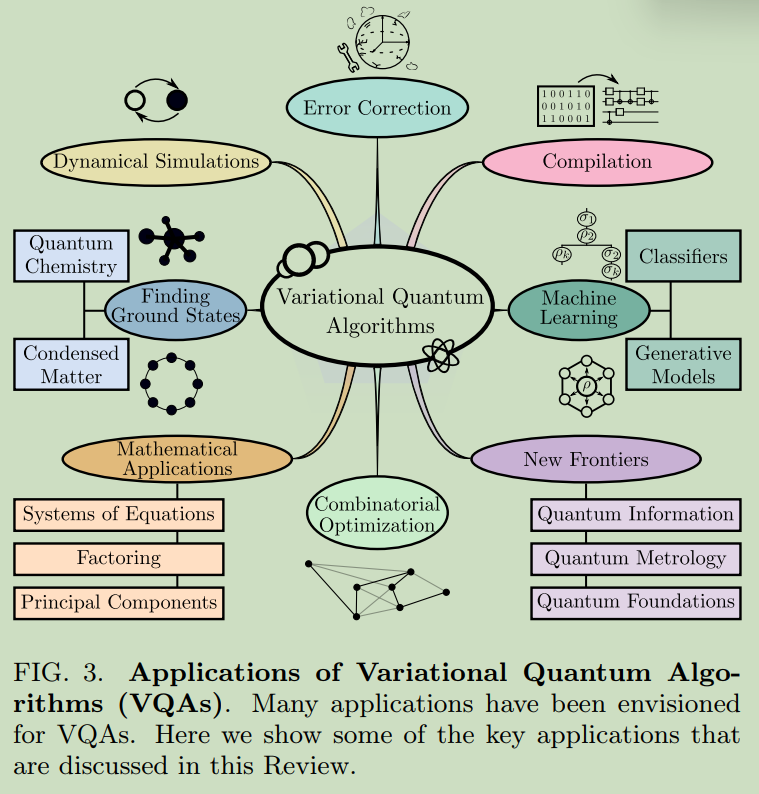
\includegraphics[width=1\linewidth]{apps-of-vqa.png}
    \caption{See \cite{cerezo2021variational}}
\end{figure}

\subsection{Parameterized Quantum Circuit (PQC) \cite{cerezo2021variational}}

In variational quantum algorithms, the optimizable parameters are defined within parameterized quantum circuits (PQCs). A PQC is a sequence of unitary operators represented by parameterized quantum gates that can be readily implemented on a quantum computer. 

Assuming we are working in an $n$-qubit Hilbert space, a parameterized quantum circuit (PQC), denoted as $U(\boldsymbol{\theta})$, can be generically expressed as the product of $L$ sequentially applied unitaries:
\begin{equation}
    U(\boldsymbol{\theta})=U_L\left(\boldsymbol{\theta}_L\right) \cdots U_2\left(\boldsymbol{\theta}_2\right) U_1\left(\boldsymbol{\theta}_1\right),
\end{equation}
with
\begin{equation}
    U_l\left(\boldsymbol{\theta}_l\right)=\prod_m e^{-i \theta_m^{l} H_m^{l}} W_m^{l}, \quad \forall l =1, \dots,L.
\end{equation}
See Fig \ref{fig:pqc}. Here, 
\begin{itemize}
    \item $W_m^{l} \in \mathbb{C}^{2^n \times 2^n}$ are fixed unparametrized unitary operators,
    \item $H_m^{l} \in \mathbb{C}^{2^n \times 2^n}$ are Hermitian operators,
    \item $\theta_m^{l}$ is the $m$-th element in $\boldsymbol{\theta}_l$,
    \item $\boldsymbol{\theta}=\left\{\boldsymbol{\theta}_1, \boldsymbol{\theta}_2, \ldots, \boldsymbol{\theta}_L \right\}$ are the parameters that we need to optimize.
\end{itemize}

\textbf{Q: Why is the $U_l\left(\boldsymbol{\theta}_l\right)$ structure designed this way? }
A: This is what can be executed by near-term quantum computers. For mathematicians, we have no choice but to accept it.

\begin{figure}
    \centering
    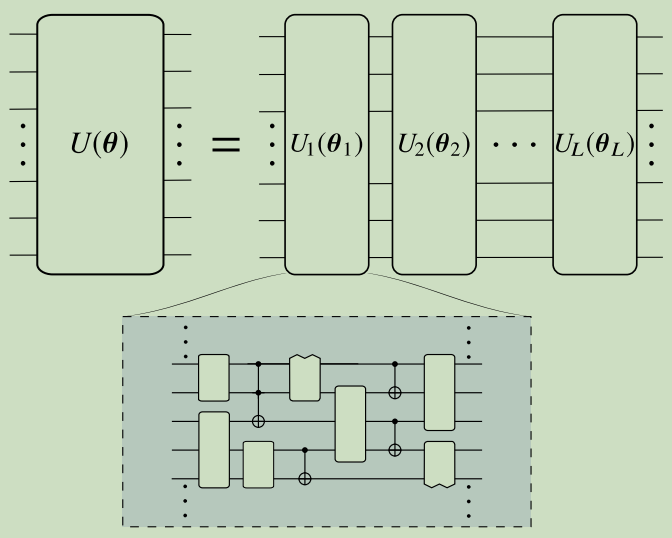
\includegraphics[width=0.75\linewidth]{Images/ansatz.png}
    \caption{Schematic diagram of an ansatz.}
    \label{fig:pqc}
\end{figure}

\subsection{Variation Quantum Eigensolvers (VQE) \cite{ding2023random}}

The variation quantum eigensolvers (VQE) finds the smallest eigenvalue (\textbf{ground state energy}) and its corresponding eigenvector (\textbf{ground state}) of a given Hamiltonian matrix $H$ by finding:
\begin{equation}
    \theta^*=\operatorname{argmin}_{\boldsymbol{\theta}} f(\boldsymbol{\theta})=\operatorname{argmin}_{\boldsymbol{\theta}}\left\langle U(\boldsymbol{\theta}) \psi_0|H| U(\boldsymbol{\theta}) \psi_0\right\rangle .
\end{equation}
Note that
\begin{enumerate}
    \item $\left|\psi_0\right\rangle \in \mathbb{C}^{2^n}$ is a predetermined initial state that can be easily prepared on a quantum computer.
    \item For each given $\boldsymbol{\theta}, U(\boldsymbol{\theta})$ is implemented on a quantum computer to evolve $\left|\psi_0\right\rangle$.
    \item The corresponding energy $f(\boldsymbol{\theta})$ and its gradient $\nabla_{\boldsymbol{\theta}} f(\boldsymbol{\theta})$ can be consequently obtained with measurements. 
\end{enumerate}

\textbf{Q: Why not directly use the quantum state as an optimization variable? Just like,}
\begin{equation}
    | \psi^*\rangle
=\operatorname{argmin}_{|\psi\rangle} \langle \psi| H | \psi\rangle.
\end{equation}
A: Our goal is to design a quantum circuit that prepares the ground state. Directly preparing this state is difficult. However, we can control the parameters of the gates. In this case, initial state is easy to prepare, and the output state we obtain is exactly what we want!

\section{Parameter-shift Rule: Analytically Estimate of Derivatives (adapted from \cite{crooks2019gradients})}

% Estimating the gradient and higher-order derivatives on quantum hardware

We consider the expectation value of a Hermitian observable $M$ measured by
\begin{equation}
    f(\boldsymbol{\theta})=\left\langle 0\left|U(\boldsymbol{\theta})^{\dagger} M U(\boldsymbol{\theta})\right| 0\right\rangle
\end{equation}
with
\begin{equation}
    U(\boldsymbol{\theta})=V_m U_m\left(\theta_m\right) \cdots V_2 U_2(\theta) V_1 U_1\left(\theta_1\right),
\end{equation}
where $V_j$ are constant arbitrary circuits, $U_j\left(\theta_j\right)$ are rotation-like gates, i.e., characterized by a Hermitian generator $H_j$ such that $H_j^2=\textbf{1}$ (involutory matrix) and so
\begin{equation}
    U_j\left(\theta_j\right)=e^{-(i / 2) H_j \theta_j}=\cos \left(\theta_j / 2\right) \textbf{1}-i \sin \left(\theta_j / 2\right) H_j .
\end{equation}

In the work \cite{crooks2019gradients}, they are interested in evaluating derivatives of an arbitrary order $d$, which we can cast as a tensor with indices $j_1, j_2, \ldots, j_d$ whose elements are the real numbers
\begin{equation}
    g_{j_1, j_2, \ldots, j_d}(\boldsymbol{\theta})=\frac{\partial^d f(\boldsymbol{\theta})}{\partial \theta_{j_1} \partial \theta_{j_2} \cdots \partial \theta_{j_d}},
\end{equation}
where the gradient and the Hessian correspond to the particular cases with $d=1$ and $d=2$, respectively.

\subsection{First-order Derivatives: The Gradient}
The result is a family of parameter-shift rules
\begin{equation}
    \label{eq:grad-shift}
g_j(\boldsymbol{\theta})=\frac{f\left(\boldsymbol{\theta}+s \mathbf{e}_j\right)-f\left(\boldsymbol{\theta}-s \mathbf{e}_j\right)}{2 \sin (s)}, \quad \forall s \neq k \pi, k \in \mathbb{Z},
\end{equation}
where $\mathbf{e}_j$ is the unit vector along the $\theta_j$ axis. Notice that 
\begin{itemize}
    \item Even if this expression looks like a finite difference approximation, it is actually exact and we can use it to analytically estimate the gradient of expectation values.
    \item It is important to remark that the formula in Eq. (\ref{eq:grad-shift}) is exact for any choice of $s$. 
\end{itemize}

\textbf{Q: why can we have this nice result?} 
A: Consider a one-qubit system. The key point is the fact that for any real constant $a$, and Hermitian operator $G$ with two unique eigenvalues, if we set
\begin{equation}
    U_H(\theta)=e^{-i a \theta H}
\end{equation}
then
\begin{equation}
    \frac{\partial}{\partial \theta} U_H(\theta)=-i a H \cdot e^{-i a \theta H} = -i a H \cdot U_H(\theta) .
\end{equation}

\subsection{Second-order Derivatives: The Hessian}
Applying the same rule twice, we get a similar formula for the Hessian,
\begin{equation}
\begin{aligned}
g_{j_1, j_2}(\boldsymbol{\theta})=[ & {\left[f\left(\boldsymbol{\theta}+s_1 \mathbf{e}_{j_1}+s_2 \mathbf{e}_{j_2}\right)-f\left(\boldsymbol{\theta}-s_1 \mathbf{e}_{j_1}+s_2 \mathbf{e}_{j_2}\right)\right.} \\
& \left.-f\left(\boldsymbol{\theta}+s_1 \mathbf{e}_{j_1}-s_2 \mathbf{e}_{j_2}\right)+f\left(\boldsymbol{\theta}-s_1 \mathbf{e}_{j_1}-s_2 \mathbf{e}_{j_2}\right)\right] \\
& \times\left[4 \sin \left(s_1\right) \sin \left(s_2\right)\right]^{-1}, \quad \forall s \neq k \pi, k \in \mathbb{Z}.
\end{aligned}
\end{equation}

\subsection{Summary}

\begin{enumerate}
    \item Unlike finite differences, it provides an exact estimate. However, similarly, we need to calculate each component of the gradient or Hessian matrix one by one.
    \item Notice that the function value $f$ itself is an expectation, which cannot be precisely evaluated. Therefore, in practice, the derivatives still cannot be obtained exactly.
    \item Essentially, those derivatives are linear combinations of multiple function values $f$.
\end{enumerate}

\section{Stochastic Gradient Descent for VQA (adapted from \cite{sweke2020stochastic})}

\subsection{Stochastic Gradient Descent (SGD)}

Given a model parameterized by $\boldsymbol{\theta} \in \mathbb{R}^d$, and some loss function $\mathcal{L}: \mathbb{R}^d \rightarrow \mathbb{R}$, stochastic gradient descent algorithms can be viewed as optimization algorithms in which the exact gradient descent update rule
\begin{equation}
    \boldsymbol{\theta}^{(t+1)}=\boldsymbol{\theta}^{(t)}-\alpha \nabla \mathcal{L}\left(\boldsymbol{\theta}^{(t)}\right),
\end{equation}
is replaced with a stochastic update rule of the form
\begin{equation}
    \boldsymbol{\theta}^{(t+1)}=\boldsymbol{\theta}^{(t)}-\alpha g^{(t)}\left(\boldsymbol{\theta}^{(t)}\right),
\end{equation}
where $\left\{g^{(t)}(\boldsymbol{\theta})\right\}$ is a sequence of random variables - estimators of the gradient - which defines the particular algorithm. A fundamental property required for obtaining convergence guarantees is that the estimators are unbiased:
\begin{equation}
    \mathbb{E}\left[g^{(t)}(\boldsymbol{\theta})\right]=\nabla \mathcal{L}(\boldsymbol{\theta})
\end{equation}
for all $t$. 

\subsection{Unbiased Estimators of Function Values}

Consider as the simplest loss function in VQA
\begin{equation}
    \mathcal{L}(\boldsymbol{\theta})=\langle O\rangle_{\boldsymbol{\theta}}:=\left\langle\mathbf{0}\left|U^{\dagger}(\boldsymbol{\theta}) OU(\boldsymbol{\theta})\right| \mathbf{0}\right\rangle,
\end{equation}
for some observable $O$.

\begin{definition}[Definition 2 ($n$-sample mean estimator)]
    Given a parameterized quantum circuit $U(\boldsymbol{\theta})$ (with $\boldsymbol{\theta} \in \mathbb{R}^d$ ) and an observable $O$ we define $\tilde{o}^{(n)}(\boldsymbol{\theta})$ as the $n$-sample mean estimator of $\langle O\rangle_{\boldsymbol{\theta}}-$ i.e., the estimator of $\langle O\rangle_{\boldsymbol{\theta}}$ obtained by averaging the results of $n$ measurements of the observable $O$ on the state vector $U(\boldsymbol{\theta})|0\rangle$.
\end{definition}

Note that by construction we have that
\begin{equation}
    \mathbb{E}\left[\tilde{o}^{(n)}(\boldsymbol{\theta})\right]=\langle O\rangle_{\boldsymbol{\theta}},
\end{equation}
for all $n$, and that while all $n$-sample mean estimators have the same expectation value the variance of the estimator decreases with increasing $n$. 

\subsection{Unbiased Estimators of Gradients}

\begin{definition}[Definition 1 (Parameter shift rule)]
    A quantum circuit $U(\boldsymbol{\theta})$ parameterized by $\boldsymbol{\theta} \in \mathbb{R}^d$, satisfies a $K$-term parameter shift rule if for all observables $O$ and for all parameters $\theta_i$, with $i \in[1, \ldots, d]$, there exist some $\left\{\gamma_{k, i}\right\}$ and $\left\{c_{k, i}\right\}$ such that
    \begin{equation}
    \frac{\partial}{\partial \theta_i}\langle O\rangle_{\boldsymbol{\theta}}=\sum_{k=1}^K \gamma_{k, i}\langle O\rangle_{\boldsymbol{\theta}_{k, i}},
\end{equation}
where $\boldsymbol{\theta}_{k, i}=\boldsymbol{\theta}+c_{k, i} \boldsymbol{e}_i$, with $\boldsymbol{e}_i$ denoting a unit vector in the $i$-th direction.
\end{definition}

Such estimators can be linearly combined to obtain unbiased estimators for derivatives, i.e.,
\begin{equation}
    \mathbb{E}\left[\sum_{k=1}^K \gamma_{k, i} \tilde{o}^{(n)}\left(\boldsymbol{\theta}_{k, i}\right)\right]=\sum_{k=1}^K \gamma_{k, i} \mathbb{E}\left[\tilde{o}^{(n)}\left(\boldsymbol{\theta}_{k, i}\right)\right]=\sum_{k=1}^K \gamma_{k, i}\langle O\rangle_{\boldsymbol{\theta}_{k, i}}=\frac{\partial}{\partial \theta_i}\langle O\rangle_{\boldsymbol{\theta}},
\end{equation}
and therefore the estimator 
\begin{equation}
    g_i(\boldsymbol{\theta}):=\sum_k \gamma_{k, i} \tilde{o}^{(n)}\left(\boldsymbol{\theta}_{k, i}\right)
\end{equation}
is an unbiased estimator for $\partial \mathcal{L}(\boldsymbol{\theta}) / \partial \theta_i$, which requires $n K$ measurements to construct. 

\subsection{Convergence Guarantees}

\begin{figure}
    \centering
    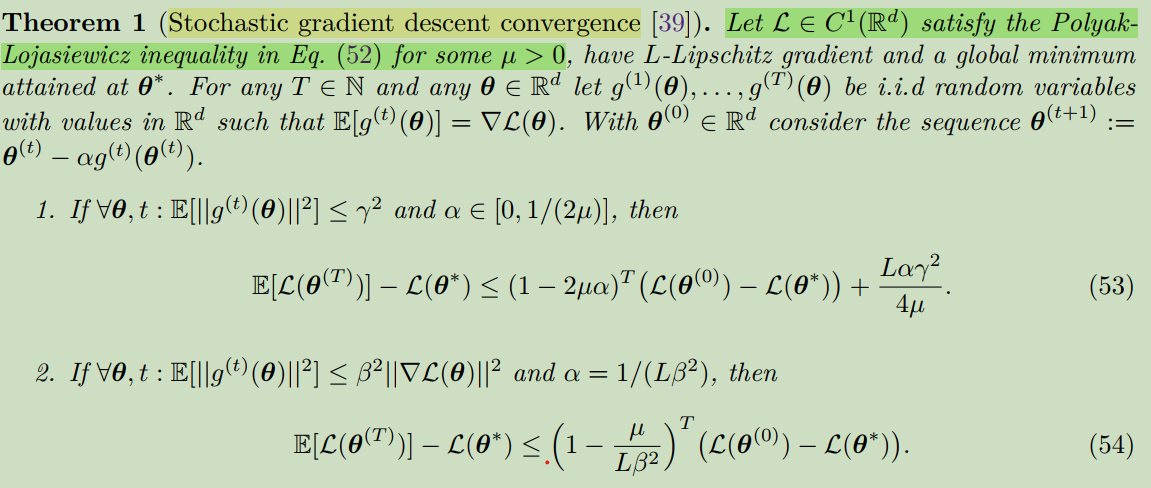
\includegraphics[width=1\linewidth]{Images/sgd-convergence.png}
    \label{fig:sgd-convergence}
\end{figure}

\textbf{Here, Polyak- Lojasiewicz (PL) inequality is an assumption.} See Fig. \ref{fig:sgd-convergence}.

\section{Random Coordinate Descent (RCD) for VQA (adapted from Ding \cite{ding2023random})}

\begin{problem}
    Problem 1 (Optimizing parameterized quantum circuits). Finding an efficient algorithm to solve the optimization problem,
\begin{equation}
    \boldsymbol{\theta}^*=\operatorname{argmin}_{\boldsymbol{\theta} \in \mathbb{R}^d} f(\boldsymbol{\theta}),
\end{equation}
under the following assumptions:
\begin{enumerate}
    \item The cost of evaluating a partial derivative scales linearly with that of a function value. (This is exactly general case of (\ref{eq:grad-shift}))
    \item Every evaluation of the function and partial derivative is susceptible to Gaussian noise:
\end{enumerate}
\begin{equation}
    f(\boldsymbol{\theta}) \rightarrow f(\boldsymbol{\theta})+N\left(0, \sigma_1^2(\boldsymbol{\theta})\right), \quad \partial_i f(\boldsymbol{\theta}) \rightarrow \partial_i f(\boldsymbol{\theta})+N\left(0, \sigma_2^2(\boldsymbol{\theta})\right)
\end{equation}
\end{problem}

\subsection{Random Coordinate Descent (RCD)}

Random Coordinate Descent (RCD) can be viewed as a variant of gradient descent (GD) where the full gradient in GD is approximated by a randomly selected component of $\nabla f\left(\boldsymbol{\theta}_n\right)$ in each iteration. Specifically, one RCD iteration can be expressed as:
\begin{equation}
    \boldsymbol{\theta}_{n+1}=\boldsymbol{\theta}_n-a_n \boldsymbol{e}_{i_n} \partial_{i_n} f\left(\boldsymbol{\theta}_n\right) .
\end{equation}
Here $\boldsymbol{e}_{i_n}$ is the $i_n$-th unit direction, $f_{i_n}^{\prime}\left(\boldsymbol{\theta}_n\right)$ is the corresponding partial derivative of the cost function, and $i_n$ is a random index uniformly drawn from $\{1,2, \cdots, d\}$. 

Similar to Eq. (6), we can write the \textbf{noisy} RCD as:
\begin{equation}
    \boldsymbol{\theta}_{n+1}=\boldsymbol{\theta}_n-a_n \boldsymbol{e}_{i_n} g_{i_n}\left(\boldsymbol{\theta}_n\right).
\end{equation}

\subsection{Main Result: Complexity Comparison of GD and RCD}

\textbf{Here, Polyak- Lojasiewicz (PL) inequality is an assumption.}
\begin{figure}
    \centering
    \includegraphics[width=1\linewidth]{table:RCD.png}
\end{figure}
\begin{figure}
    \centering
    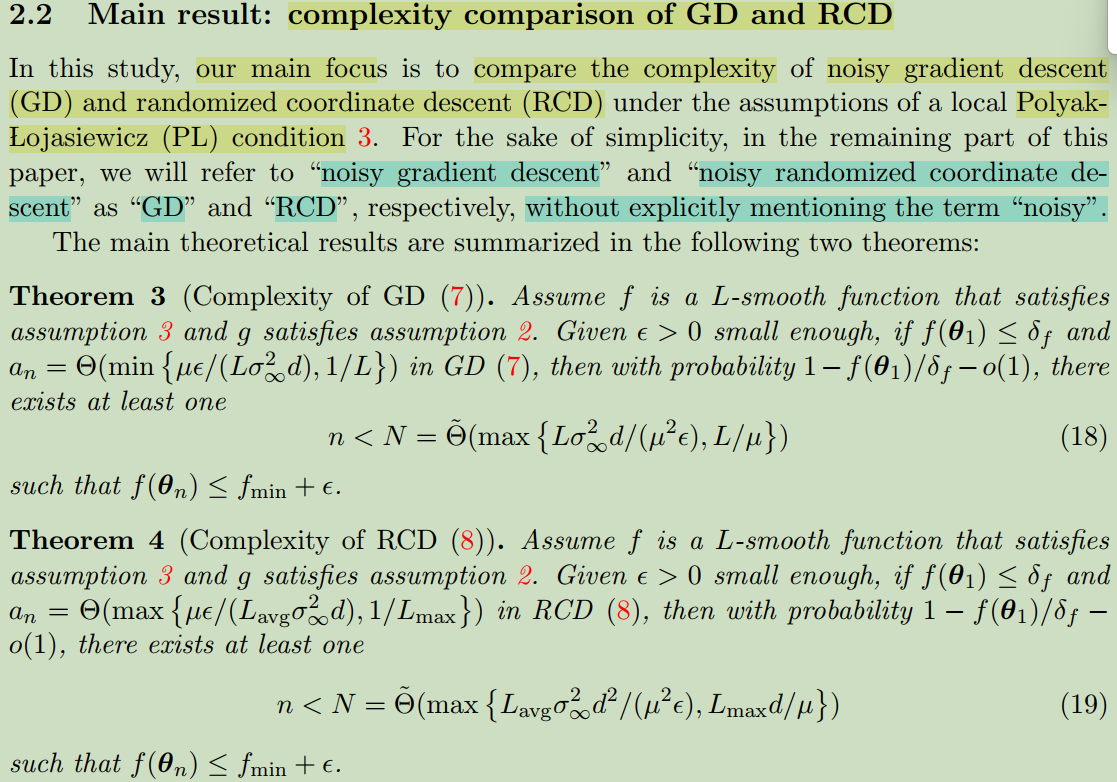
\includegraphics[width=1\linewidth]{main-results.png}
\end{figure}

%----------------------------------------------------------------------------------------
%	Bibliography
%----------------------------------------------------------------------------------------

\chapter{Bibliography}
\markboth{\sffamily\normalsize\bfseries Bibliography}{\sffamily\normalsize\bfseries Bibliography} % Set the page headers to display a Bibliography chapter name
\addcontentsline{toc}{chapter}{\textcolor{ocre}{Bibliography}} % Add a Bibliography heading to the table of contents

\section{Articles}
\addcontentsline{toc}{section}{Articles} % Add the Articles subheading to the table of contents

\printbibliography[heading=bibempty, type=article] % Output article bibliography entries

\section{Books}
\addcontentsline{toc}{section}{Books} % Add the Books subheading to the table of contents

\printbibliography[heading=bibempty, type=book] % Output book bibliography entries

%----------------------------------------------------------------------------------------
%	INDEX
%----------------------------------------------------------------------------------------

\cleardoublepage % Make sure the index starts on an odd (right side) page
\phantomsection
\addcontentsline{toc}{chapter}{\textcolor{ocre}{Index}} % Add an Index heading to the table of contents
\printindex % Output the index

%----------------------------------------------------------------------------------------
%	APPENDICES
%----------------------------------------------------------------------------------------

\chapterimage{orange2.jpg} % Chapter heading image
\chapterspaceabove{6.75cm} % Whitespace from the top of the page to the chapter title on chapter pages
\chapterspacebelow{7.25cm} % Amount of vertical whitespace from the top margin to the start of the text on chapter pages

%----------------------------------------------------------------------------------------

\end{document}

